\documentclass[12pt,a4paper]{article}
\usepackage[T1]{fontenc}
\usepackage[utf8]{inputenc}
\usepackage{amsmath,amssymb,amsfonts,amsthm,mathtools}
\usepackage{graphicx,float,geometry,hyperref,enumitem,xcolor}
\usepackage{listings}
\geometry{margin=2.5cm}

% Theorem environments
\theoremstyle{definition}
\newtheorem{definition}{Définition}[section]
\newtheorem{exemple}{Exemple}[section]
\theoremstyle{plain}
\newtheorem{theoreme}{Théorème}[section]
\newtheorem{proposition}{Proposition}[section]
\theoremstyle{remark}
\newtheorem{remarque}{Remarque}[section]

% Macros
\newcommand{\SC}{\text{S.C.}}
\newcommand{\jeton}{\texttt{jeton}}
\newcommand{\tampon}{\texttt{tampon}}
\newcommand{\estampille}{\texttt{estampille}}
\newcommand{\demande}{\texttt{demande}}
\newcommand{\dedans}{\texttt{dedans}}
\newcommand{\requete}{\texttt{requête}}

% Pseudocode style
\lstset{
  basicstyle=\small\ttfamily,
  breaklines=true,
  frame=single,
  xleftmargin=1em,
  xrightmargin=1em,
  backgroundcolor=\color{gray!8},
  escapeinside={(*}{*)},
}

\title{\textbf{Cours 7 --- Algorithmique Distribuée et Parallélisme}\\
\large Exclusion mutuelle distribuée et élection sur anneau}
\author{Notes de cours --- 18/02/26}
\date{}

\begin{document}
\maketitle
\tableofcontents
\newpage

%──────────────────────────────────────────────────────────
\section{Algorithme de Lamport --- Exclusion mutuelle}
%──────────────────────────────────────────────────────────

\subsection{Variables et constantes (pour le processus $P_\kappa$)}

Chaque processus $P_\kappa$ maintient les variables suivantes :

\begin{itemize}[leftmargin=2em]
  \item \textbf{Constante :} \texttt{numéro}, initialisé à $\kappa$.
  \item \textbf{Variables :}
  \begin{itemize}
    \item \tampon, \demande\ : de type \jeton ;
    \item \estampille\ : horloge (entier), initialisée à $0$ ;
    \item \texttt{jeton\_présent} : booléen, initialisé à $(\texttt{mon\_numéro} = 1)$ ;
    \item \dedans\ : booléen, initialisé à \texttt{faux} ;
    \item \requete\ : message.
  \end{itemize}
\end{itemize}

\subsection{Lors de la demande d'entrée en S.C.}

\begin{lstlisting}[caption={Demande d'entrée en section critique}]
si jeton_present = faux alors
  debut
    estampille := estampille + 1;
    requete.date := estampille;
    requete.emetteur := mon_numero;
    diffuser(requete);
    attendre_jeton(tampon);
  fin
jeton_present := vrai;
dedans := vrai;
\end{lstlisting}

\subsection{Lors de la sortie de S.C.}

\begin{lstlisting}[caption={Sortie de section critique}]
var j : entier site;
tampon(mon_numero) := estampille;
dedans := faux;
pour j := mon_numero+1 jusqu'a n, 1 jusqu'a mon_numero-1
faire:
  si demande(j) > tampon(j) et jeton_present alors
    | jeton_present := faux;
    | envoyer(tampon, j);
\end{lstlisting}

\subsection{Lors de l'arrivée d'une requête}

\begin{lstlisting}[caption={Réception d'une requête}]
var h : numero;
k := requete.emetteur;
demande[k] := max(demande[h], requete.date);
si jeton_present et dedans = faux alors
  { (* envoyer le jeton *) }
\end{lstlisting}

\begin{remarque}
  La condition \texttt{jeton\_présent et dedans = faux} est vérifiée
  aussi lorsqu'on reçoit une demande \og périmée \fg{} (note de cours :
  \emph{aussitôt qu'il reçoit une demande \og périmée \fg{}}).
\end{remarque}

\subsection{Complexité et propriétés}

\begin{proposition}
  La complexité en messages est $(n-1)+1 = n$ messages par entrée en $\SC$.
\end{proposition}

\begin{proposition}[Exclusion mutuelle]
  La possession du jeton est une condition \emph{nécessaire et suffisante}
  pour entrer en section critique. L'unicité du jeton garantit l'exclusion mutuelle.
\end{proposition}

\begin{proposition}[Fairness]
  L'algorithme réalise une \emph{exploration circulaire} : chaque processus
  finit par entrer en $\SC$.
\end{proposition}

%──────────────────────────────────────────────────────────
\section{Algorithme de Lamport --- Complexité détaillée}
%──────────────────────────────────────────────────────────

Pour une entrée en $\SC$, le nombre de messages émis se décompose en trois termes :
\[
  \underbrace{(n-1)}_{\text{diffusion demande}}
  + \underbrace{(n-1)}_{\text{diffusion sortie}}
  + \underbrace{(n-1)}_{\text{acquittements}}
  = 3(n-1).
\]
En graphe complet, la diffusion est directe : chaque message coûte $1$ saut,
soit un total en $O(n)$. Sur un anneau ou un graphe quelconque, chaque diffusion
peut nécessiter jusqu'à $n-1$ sauts, ce qui porte le coût global à $O(n^2)$.

\begin{figure}[H]
  \centering
  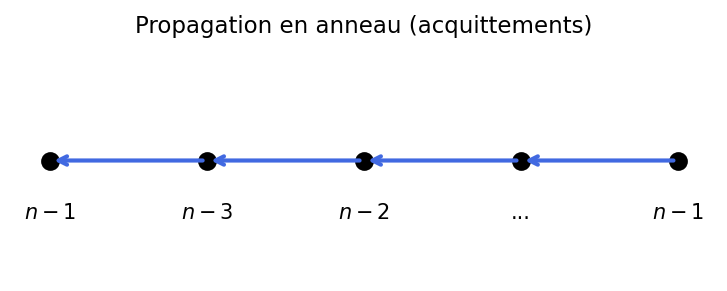
\includegraphics[width=0.65\textwidth]{figures/fig_ring_propagation.png}
  \caption{Propagation des acquittements le long de l'anneau (de $n-1$ à $n-2$, etc.)}
  \label{fig:ring_propagation}
\end{figure}

%──────────────────────────────────────────────────────────
\section{Algorithme de Ricart et Agrawala}
%──────────────────────────────────────────────────────────

\subsection{Principe}

\begin{definition}[Privilège implicite]
  Un processus a le \emph{privilège} d'entrer en $\SC$ s'il possède la
  plus petite estampille parmi toutes les demandes en cours.
\end{definition}

L'exclusion mutuelle est assurée par :
\begin{itemize}
  \item Seul un processus avec la plus petite estampille peut entrer en $\SC$
        (algorithme + canaux FIFO) ;
  \item La plus petite demande est unique (horloge de Lamport élargie).
\end{itemize}

\begin{proposition}[Fairness]
  Le processus avec la plus petite estampille finit toujours par entrer en $\SC$,
  pourvu qu'il n'y ait ni perte de message ni blocage.
  Le nombre de processus \og précédant \fg{} le processus candidat vérifie :
  (i)~$k < n-1$ (par l'algorithme) et (ii)~$k$ décroît d'au moins $1$ au bout
  d'un certain temps.
\end{proposition}

\subsection{Du privilège implicite au jeton}

Dans l'algorithme de Lamport, le privilège est \emph{implicite} (condition sur
les estampilles). Ricart--Agrawala rend ce privilège \emph{explicite} via un
objet appelé \textbf{jeton}.

\begin{definition}[Jeton]
  Le \jeton\ est un tableau indexé par les sites, contenant pour chaque processus
  le nombre de fois qu'il est entré en $\SC$ (horloge interne).
  Exemple : $\jeton = [2 \mid 0 \mid 5 \mid 8]$.
\end{definition}

Propriétés du jeton :
\begin{itemize}
  \item Il est unique dans le système.
  \item Au départ, il est placé dans un processus particulier, toutes ses cellules
        valant $0$.
  \item Lorsqu'un processus libère le jeton à la sortie de $\SC$, il incrémente
        sa cellule dans le tableau.
  \item La possession du jeton garantit l'entrée en $\SC$ ;
        une entrée en $\SC$ est impossible sans le jeton.
  \item L'unicité du jeton garantit l'exclusion mutuelle.
\end{itemize}

\subsection{Diffusion de la demande et transfert du jeton}

Un processus souhaitant entrer en $\SC$ diffuse un message de demande portant
le compteur de ses entrées passées en $\SC$.

\begin{figure}[H]
  \centering
  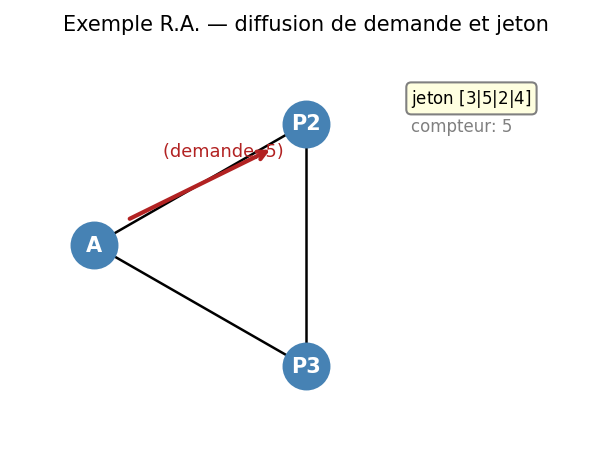
\includegraphics[width=0.55\textwidth]{figures/fig_ra_token_example.png}
  \caption{Exemple : $A$ envoie \texttt{(demande, 5)} à $P_2$ qui détient le jeton
           $[3\mid5\mid2\mid4]$ ; puis $A$ envoie \texttt{(demande, 6)} et
           $P_2$ transfère le jeton (graphe connexe).}
  \label{fig:ra_token}
\end{figure}

\subsection{Structure des données (pseudo-code)}

\begin{lstlisting}[caption={Déclarations pour l'algorithme R.A. avec jeton}]
message = (entier, emetteur);
jeton   = tableau [site] de entier;

procedure attendre_jeton(v : jeton)
  (* attend l'arrivee d'un message de type jeton
     et range sa valeur dans la variable v *);

tampon : jeton;  (* copie locale du jeton *)
\end{lstlisting}

%──────────────────────────────────────────────────────────
\section{Élection sur un anneau}
%──────────────────────────────────────────────────────────

\begin{definition}[Élection]
  Le problème d'élection consiste à désigner un processus particulier
  (\emph{leader}) parmi des processus numérotés.
\end{definition}

\textbf{Spécialisation :}
\begin{itemize}
  \item \emph{Fairness} : l'algorithme se termine explicitement.
  \item \emph{Safety} : jamais $2$ leaders simultanément, et exactement $1$ leader
        à la terminaison.
\end{itemize}

Le graphe est en forme d'\textbf{anneau}, pouvant être :
\begin{itemize}
  \item \emph{Unidirectionnel} : chaque processus connaît son successeur.
  \item \emph{Bidirectionnel} : chaque processus connaît successeur et prédécesseur.
  \item \emph{Orienté} : l'anneau est orienté ssi, pour tout couple de voisins
        $p_i$ et $p_j$ :
        \[
          \texttt{mon\_successeur}(p_i) = p_j
          \iff
          \texttt{mon\_prédécesseur}(p_j) = p_i.
        \]
\end{itemize}

\begin{remarque}
  L'\textbf{algorithme de Chang et Roberts} est un algorithme classique d'élection
  sur anneau unidirectionnel.
\end{remarque}

%──────────────────────────────────────────────────────────
\section{Exemple de déroulement --- Algorithme de Lamport}
%──────────────────────────────────────────────────────────

\textbf{Contexte :} trois processus $P_1$, $P_2$, $P_3$ en anneau triangulaire.
$P_1$ et $P_2$ demandent à entrer en $\SC$ ; $P_3$ ne demande pas à entrer.

\subsection{État initial}

\begin{figure}[H]
  \centering
  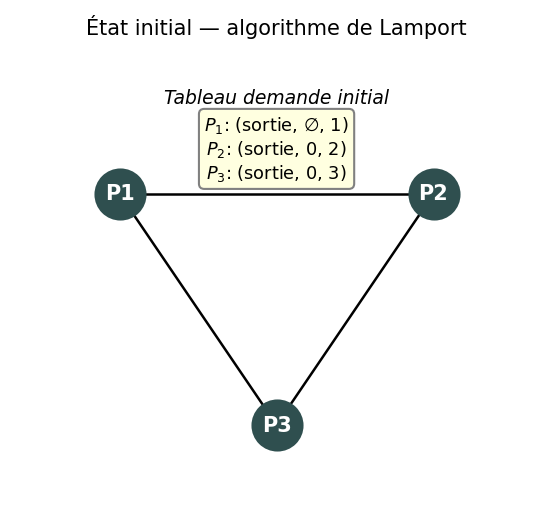
\includegraphics[width=0.45\textwidth]{figures/fig_lamport_step1.png}
  \caption{État initial du tableau \texttt{demande} :
           $P_1 = (\text{sortie}, \emptyset, 1)$,
           $P_2 = (\text{sortie}, 0, 2)$,
           $P_3 = (\text{sortie}, 0, 3)$.
           $P_2$ attend d'être le plus petit avant d'entrer.}
  \label{fig:lam_step1}
\end{figure}

\subsection{Diffusion des demandes}

$P_1$ et $P_2$ diffusent simultanément leurs requêtes.
Les canaux étant FIFO, l'ordre des demandes est conservé.

\begin{figure}[H]
  \centering
  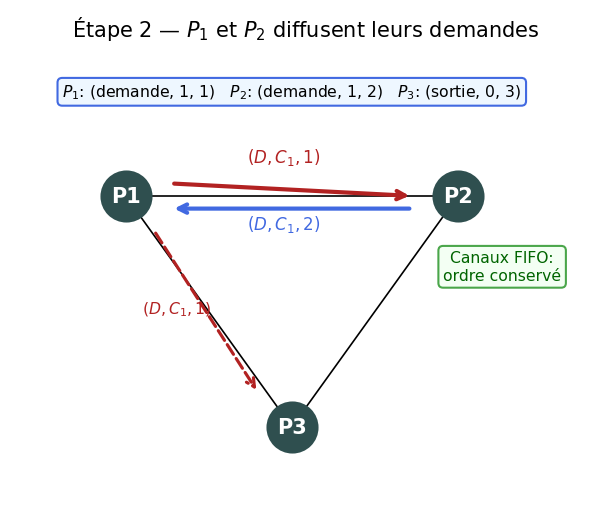
\includegraphics[width=0.52\textwidth]{figures/fig_lamport_step2.png}
  \caption{Échange de messages :
           $P_1 \to P_2$ : $(D, C_1, 1)$ et $P_2 \to P_1$ : $(D, C_1, 2)$.
           Tableau après réception :
           $P_1 = (\text{demande}, 1, 1)$,
           $P_2 = (\text{demande}, 1, 2)$,
           $P_3 = (\text{sortie}, 0, 3)$.}
  \label{fig:lam_step2}
\end{figure}

\subsection{Acquittements et entrée de $P_1$ en $\SC$}

Après réception de tous les acquittements, $P_1$ possède la plus petite
estampille (1 < 2) et entre en $\SC$. $P_2$ reste bloqué.

\subsection{Sortie de $P_1$ et entrée de $P_2$}

$P_1$ sort de $\SC$ et diffuse \texttt{sortie(4,1)}. $P_2$ reçoit ce message
et peut alors entrer en $\SC$.

\begin{figure}[H]
  \centering
  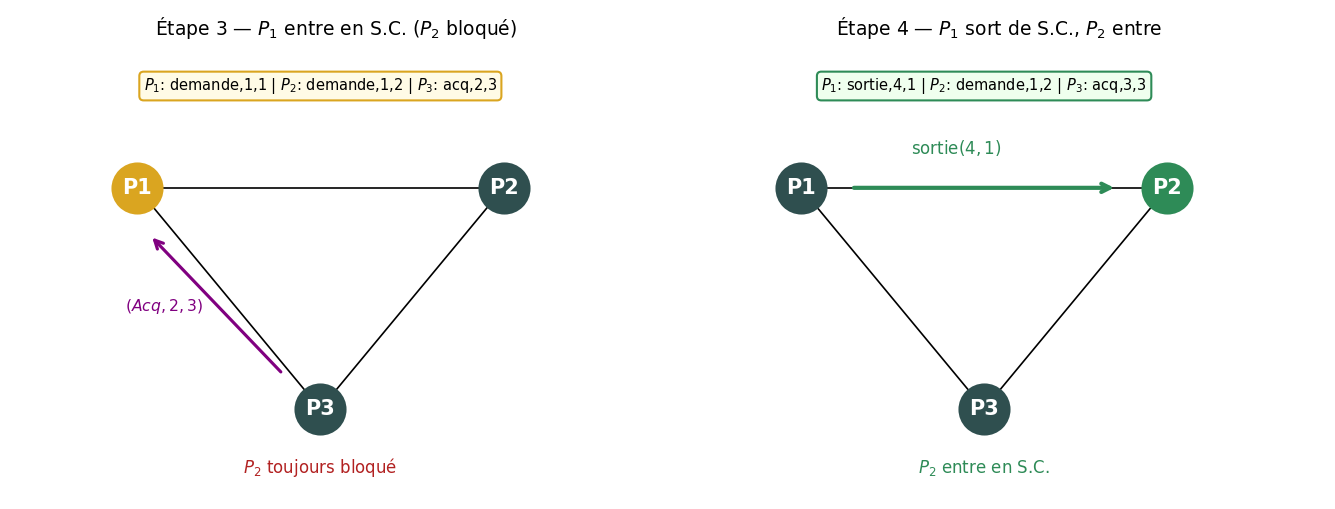
\includegraphics[width=0.92\textwidth]{figures/fig_lamport_steps34.png}
  \caption{Gauche : $P_1$ (en or) entre en $\SC$, $P_2$ reste bloqué ;
           $P_3$ envoie $(Acq, 2, 3)$ à $P_1$.
           Droite : $P_1$ sort et envoie $\text{sortie}(4,1)$ à $P_2$ (vert) ;
           $P_2$ entre en $\SC$.}
  \label{fig:lam_steps34}
\end{figure}

\end{document}
